%% -----------------------------------------------------------------
%% This file uses UTF-8 encoding
%%
%% For compilation use following command:
%% latexmk -pdf -pvc -bibtex --shell-escape thesis
%%
%% -----------------------------------------------------------------
%%                                     _     _      
%%      _ __  _ __ ___  __ _ _ __ ___ | |__ | | ___ 
%%     | '_ \| '__/ _ \/ _` | '_ ` _ \| '_ \| |/ _ \
%%     | |_) | | |  __/ (_| | | | | | | |_) | |  __/
%%     | .__/|_|  \___|\__,_|_| |_| |_|_.__/|_|\___|
%%     |_|                                          
%%
%% -----------------------------------------------------------------

\documentclass{kithesis}

% Additional packages
\usepackage[english,slovak]{babel}
\usepackage{blindtext}  % lorem ipsum
\usepackage{minted}

% Variables
%\thesisspec{figures/thesisspec.png} 

\title{Music Visualizer}{Vizualizácia hudby}

\author{Marián Sabat}
\supervisor{Ing. Norbert Ádám, PhD.} %veduci prace
%\consultant{Donald E. Knuth} %konzultant
%\college{University of Žilina}{Žilinská univerzita} %univerzita
%\faculty{Faculty of Electrical Engineering and informatics}{Fakulta elektrotechniky a informatiky} %fakulta
%\department{Department of Computers and Informatics}{Katedra počítačov a informatiky} %katedra
%\departmentacr{DCI}{KPI} % skratka katedry
%\thesis{Master thesis}{Diplomová práca} %typ prace
\submissiondate{25}{5}{2018}
%\fieldofstudy{9.2.1 Informatika}
%\studyprogramme{Informatika}
%\city{Košice} %mesto
\keywords{%\LaTeX, programming, typesetting}{\LaTeX, programovanie, sadzba textu}
}
%\declaration{som nepodvadzal}

\abstract{
    % english 
	%\blindtext
	ABSTRAKT
}{
    % slovak 
	%\blindtext
	ABSTRAKT
}

\acknowledgment{%Na tomto mieste by som rád poďakoval svojmu vedúcemu práce za jeho čas a odborné vedenie počas riešenia mojej záverečnej práce.

%Rovnako by som sa rád poďakoval svojim rodičom a priateľom za ich podporu a povzbudzovanie počas celého môjho štúdia.
    
%V neposlednom rade by som sa rád poďakoval pánom {\it Donaldovi E. Knuthovi} a {\it Leslie Lamportovi} za typografický systém \LaTeX, s ktorým som strávil množstvo nezabudnuteľných večerov.
}

\addbibresource{chapters/bibliography.bib}

% if you want to work only on selected chapters
%\includeonly{chapters/analyza} %,chapters/synteza}

% Load acronyms
\newacronym{ny}{NY}{New York}
\newacronym{la}{LA}{Los Angeles}
\newacronym{un}{UN}{United Nations}
\newacronym{gcd}{GCD}{Greatest Common Divisor}
\newacronym{lcm}{LCM}{Least Common Multiple}


%% -----------------------------------------------------------------
%%          _                                       _   
%%       __| | ___   ___ _   _ _ __ ___   ___ _ __ | |_ 
%%      / _` |/ _ \ / __| | | | '_ ` _ \ / _ \ '_ \| __|
%%     | (_| | (_) | (__| |_| | | | | | |  __/ | | | |_ 
%%      \__,_|\___/ \___|\__,_|_| |_| |_|\___|_| |_|\__|
%%                                                      
%% -----------------------------------------------------------------

\begin{document}
%% Title page, abstract, declaration etc.:
\frontmatter{}

%% List of code listings, if you are using package minted
%\listoflistings

\pagenumbering{arabic}

%% Chapters
% !TEX root = ../thesis.tex

\chaptermark{Úvod}
\addcontentsline{toc}{chapter}{Úvod}

\chapter*{Úvod}

Systémy, ktoré sa dokážu učiť z dát sú už dnes prístupné verejnosti. Je čoraz jednoduchšie študovať techniky strojového učenia a preto progres v tomto odvetví je skutočne viditeľný. Množstvo dát a dobrá výpočtová technika majú za následok, že v takmer všetkých oblastiach sa zavádza nejaký druh umelej inteligencie. Počítače, ktoré by rozumeli informáciám by znamenali revolúciu v našich životoch. Program, ktorý by dokázal vygenerovať obraz na základe hudobného podkladu, na základe emócií a nálad, ktoré sú obsiahnuté v hudbe by bol pokrok ku umelej inteligencii, ktorá by skutočne rozumela dátam.

Proces syntézy jedného druhu informácií na iní je pre ľudí prirodzený no pre stroj je to neľahká úloha. Avšak progres v neurónových sieťach a v generatívnych algoritmoch umožňuje klasifikáciu jednej informácie a jej následnú zmenu na inú formu. Stále ale existuje množstvo prekážok v realizácií tohto problému.

To všetko nás privádza k otázke, sú dnešné neurónové siete schopné previesť hudobnú skladbu na zmysluplný obraz?
Prevod hudobnej informácie na obrazovú si vyžaduje určitý stupeň kreativity a znalostí. 
V našej práci sa budeme snažiť zodpovedať tento problém.
Budeme sa snažiť vytvoriť model, ktorý by simuloval ľudskú kreativitu.

V prvom rade je dôležité upraviť dáta, ktoré budeme analyzovať. Ide o zvukové signály, ktoré ako také sú nespracovateľné dnešnými algoritmami strojového učenia.
Je nevyhnutné aby sme tieto dáta upravili na použiteľnú formu.
Ďalším krokom je zistenie či sú počítače vôbec schopné priradenia najjednoduchšej obrazovej formy, čiže farby, k hudobným skladbám.
Úspešné splnenie tejto úlohy bude dobrým predpokladom pre vytvorenie finálneho modelu, ktorý dokáže generovať obrázky na vyššej kreatívnej úrovni.

Naša práca je preto rozdelená presne podľa týchto celkov.
Prvé kapitoly poskytnú súčasné úspechy v syntéze dát a teoretický základ pre naše riešenie.
V ďalších kapitolách postupne prejdeme naše výsledky od najjednoduchších modelov až po tie zložitejšie.
Na konci poskytneme porovnanie nami vytvorených systémov a odvodenie záverov.  

% !TEX root = ../thesis.tex

\chapter{Formulácia úlohy}

%Text záverečnej práce musí obsahovať\/ kapitolu s~formuláciou úlohy resp. úloh riešených v~rámci záverečnej práce. V~tejto časti autor rozvedie spôsob, akým budú riešené úlohy a~tézy formulované v~zadaní práce. Taktiež uvedie prehľad podmienok riešenia.

% !TEX root = ../thesis.tex

\chapter{Syntéza dát}
\label{synteza_dat}

Už od čias pred počítačmi ľudia využívali abstrakciu skutočných dát v podobe čísel a matematiky. S vývojom výpočtovej techniky prišli aj nové spôsoby zmeny jedného typu informácií na iný. Dnes existuje mnoho systémov určených na tento proces.

\section{Zmena textu na reč}
Už v osemdesiatych rokoch dvadsiateho storočia, keď Steve Jobs predstavil nový Macintosh, počítač vedel hovoriť.
Systémy, ktoré používajú zmenu textu na reč sú dnes bežná vec, a preto je ťažké predstaviť si svet bez nich \cite{text2speech}.
Aj keď sú zaužívané stále existuje priestor na zlepšenie. Hlas starého Macintosha bol zreteľne umelý, no dnes existujú programy, ktoré dokážu simulovať ľudskú reč takmer na nerozpoznanie od živých ľudí.
Tieto syntetizátory našli svoje využitie napríklad v telekomunikáciách.
Primitívne úlohy vykonávané cez telefón sú zverené počítačom.
Ľudia si už zvykli, že keď volajú niekam aby si niečo vybavili je normálne ak sa im ozve stroj.
Syntetizátory našli svoje využitie aj vo vzdelávaní.
Učenie jazykov z pohodlia domova je možné aj vďaka tomu, že počuť ako sa slovo vyslovuje môžeme bez prítomnosti skúseného rečníka či cudzinca.
Zrakovo postihnutí práve vďaka technológií zmeny textu na reč môžu využívať prístroje, ako napríklad počítače, telefóny a iné,  bez ktorých sa dnes už nezaobídeme.
Nie len slepím, ale aj nemým a inak telesne postihnutým pomáhajú čítačky textu každý deň. Svoje využitie našli v mnohých oblastiach od vedy a výskumu až po zábavný priemysel.

\section{Prevod reči na text}
Pre ľudí veľmi jednoduchá úloha, rozpoznanie reči, je pre číselné systémy netriviálna záležitosť.
Fourierové transformácie a úprava dát nám dávajú šancu na extrakciu vhodných informácií, ktoré sa stali vhodným nástrojom na detekciu slov \cite{speechRecognition}.
Systém schopný prevodu hovorenej reči na text je nevyhnutnosťou v prípadoch, keď človek nemôže alebo nedokáže použiť klávesnicu či iní mechanický vstup.
Osobní asistenti ako Cortana alebo Ok Google by bez týchto syntetizátorov nedosiahli takej popularity.
Prevodníky reči na text majú veľký vplyv na to ako pracujeme s našimi zariadeniami. Funkcie ako preklad z jedného jazyka do druhého v reálnom čase sa zavádzajú do programov určených na komunikáciu a zmenšujú tak priepasť medzi ľuďmi rôznych národností.
To by nebolo možné ak by jadrá týchto programov nestáli na technológiách prevodu reči na text a textu na reč.

\section{Rozpoznávanie obsahu dát}
S úlohou syntézy informácií súvisí aj problém reprezentovania významu dát.
Naučiť počítače rozpoznávať čo sa nachádza na obrázku je dnes silno skúmaná oblasť.
Mnohé automobilové spoločnosti sa snažia vytvoriť samo jazdiace vozidlá, ktoré dokážu spozorovať prekážky okolo seba a zareagovať rýchlejšie ako by to dokázal ktorýkoľvek človek.
Vďaka najnovším metodikám, ako napríklad využite konvolučných neurónových sietí,  ľudia vytvorili programy, ktoré dokážu rozpoznať čo sa nachádza na obrázkoch a rozoznať jednotlivé objekty \cite{tensorFlow}.
Takéto technológie sa dajú využiť napríklad pri vyhľadávaní. Spoločnosti ako Google ponúkajú cloudové služby stvorené presne na tieto účely \cite{googleCloud}.

Neurónové siete dokážu analyzovať obrázky na úrovniach aké doposiaľ neboli možné.
V roku 2016 výskumníci z Montrealu a Toronta vytvorili model, ktorý dokázal analyzovať obrázky a vytvoriť textový popis týkajúci sa obsahu obrázku \cite{imageCaption}.
V spojení s čítačkou textu by sme takto mohli ešte viac uľahčiť prístup k informáciám aj pre zdravotne postihnutých ale aj využiť takúto technológiu na ešte lepšie výsledky.
Detekcia tvári sa zavádza aj do mobilných telefónov a využíva sa na odomykanie uzamknutej obrazovky. Facebook vytvára systém, ktorý by využil rozpoznanie tváre a využil tieto dáta ako heslo pre používateľa \cite{facebook}.
Analýza obrazu ale neostáva len pri rozpoznávaní objektov. Inteligentné systémy dokážu rozpoznať rôzne vlastnosti obrazu.
Google vytvoril systém, ktorý nazval Deep dream. Deep dream dokáže rozpoznať vlastnosti obrazu a upraviť pôvodný obrázok pridaním vrstiev, ktoré majú podobné vlastnosti.
Vytvorené obrázky potom vyzerajú ako halucinácie.
Mnohé iné webové aplikácie zase využívajú siete, ktoré sa naučia ako rozpoznať štýl obrazu a vďaka tomu dokážu preniesť štýl na úplne iný obrázok. Vznikajú tak zaujímavé filtre na úpravu obrázkov a fotiek. 

\section{Generovanie obrázkov}
V posledných rokoch systémy strojového učenia preukazujú výsledky v generovaní nových dát.
Syntéza textu na obraz je jednou z najnovších prác v tomto odvetví \cite{text2image}.
Nakoľko ide o experiment, tak komerčné využitie ešte neexistuje. Ale pri zlepšení tejto technológie sa môže vytvoriť obrovský potenciál.
Takéto výskumy prebiehajú na celom svete a na prechod na trh určite nebudeme dlho čakať.
Umelo generované obrázky dokážeme vďaka tomu ako sú vytvorené ďalej upraviť.
Nakoľko sú to obrázky vytvorené pomocou matematického modelu vieme upravovať obsah veľmi jednoducho.
Príkladom sú generované obrázky ľudí, v ktorých sa dá upravovať napríklad to či sa osoba usmieva alebo nie, či má okuliare alebo mnoho iných vlastnosí \cite{DCGAN}.

\chapter{Teoretický základ}
\label{teoreticky_zaklad}

Ako už bolo avizované naša práca sa zaoberá neurónovými sieťami. Preto v tejto kapytole zhrnieme základné pojmi a problémi, pred ktorými stojíme.

Algoritmus, ktorý sa učí z dát, poskituje dobé výsledky len vtedy ak má dobré dáta, z ktorých sa učí. 
Náš model sa bude učiť z hudobných dát.
Zvukové analógové sygnály uložené v digitálnej forme sú príliš rozsiahle nato aby sme ich mohli využiť ako vstup do neurónovej siete.
Jedinou možnosťou je úprava takýchto dát na jednoduchšiu formu.

\section{Hudobné dáta}
Ľudia vnímajú hudbu na rôznych úrovňach.
Rôzne vlastnosti harmonických zvukov vyvolávajú u nás rozličné emócie.
Napríklad kým vzrušenie blízko súvisí s tempom, tak výška tónov a hlasitosť skôr určujú náladu skladby \cite{emotionExtraction}.
To ako vnímame hudbu má preto veľký pliv na našu predstavivosť.

Hudobné dáta sú ľahko dostupné na internete. Čo sa týka hudby existuje niekoľko zdrojov pre informácie \cite{musicMining}:
\begin{itemize}
	\item Hudobné metadáta,
	\item Akustické vlastnosti,
	\item Slová,
	\item Hudobná kritika,
	\item MIDI súbory,
	\item Hudobné skóre.
\end{itemize}
Rôzne typy informácií majú využitie v rôznych prípadoch.
Nás budú zaujímať akustické vlastnosti, medzi ktoré patrí energia, rytmus, časové a spektrálne vlastnosti \cite{emotionExtraction}.
Pre každú z týchto sád vlastností existuje niekoľko vlastnosí, ktoré sa dajú extrahovať známimi algoritmami a programmi.
V tabuľke 2.1 sme uviedli zopár významných údajov, ktoré by sme mohli využiť pre trénovanie naších modelov.
Tieto údaje opisujú hudobnú informáciu a majú značne menšiu veľkosť ako skladba uložená vo formáte mp3 alebo wav.

\begin{table}[]
\centering
\caption{Akustické vlastnosti zvukových sygnálov}
\label{features_table}
\begin{tabular}{l p{10cm}}
\hline
\textbf{Sada vlastností} & \textbf{Extrahovateľné vlastnosti}                                                                                                                                                                             \\ \hline
Energia                  & Dynamická hlasitosť, výkon zvuku, celková hlasitosť, špecifické koeficienty citlivosti na hlasitosť                                                                  \\
Rytmus                   & Diagram úderov, vzor rytmu, histogram rytmu a tempo, sila rytmu, pravidelnosť rytmu, jasnosť rytmu, priemerná frekvencia nástupu, priemerné tempo                  \\
Časové vlastnosti        & Nulové priechody, logaritmus času útoku                                                                                                                                                                        \\
Spektrálne vlastnosti    & Spektrálne centroidy, spektrálne vyhodnocovanie, spektrálny tok, spektrálne merania rovinnosti, spektrálne hrudkové faktory, mel-frekvenčné kepstrálne koeficienty \\
Harmónia                 & Jasnosť kľúča, hudobný režim, harmonická zmena, diagram stúpania                                                                                                     \\ \hline
\end{tabular}
\end{table}

\section{Neurónové siete}
Tak ako mozog, neurónová sieť je spojenie viacerých neurónov do siete.
Neurón na vstupe príma informácie, ktoré pozmení a pošle na výstup, čo môže byť vstup ďalšieho neurónu.

Formálny neurón alebo perceptrón (obrázok 2.1) má na vstupe \(n\) aktivít \cite{NNKvasnicka}.
Označme vstup ako vektor \(x = (x_1, x_2, x_3, ... x_n)^T\), kde \(T\) označuje transponovaný vektor.

\begin{figure}[!ht] 
	\centering 
	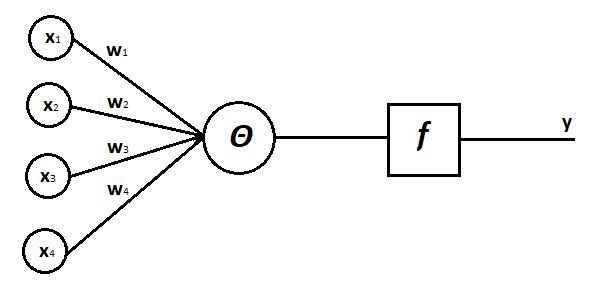
\includegraphics[width=.6\textwidth]{figures/perceptron} 
	\caption{Model formálneho neurónu.} 
\end{figure}

Všetky vstupné kanály majú svoju váhu, označme preto váhy vstupov ako vektor \(w = (w_1, w_2, w_3, ... w_n)^T\).
Celkový vstup perceptrónu sa potom vypočíta ako súčet súčinu vektorov \(x\) a \(w\), a prahu excitácie \(\Theta\).
Pre získanie výstupu vstupy prejdú aktivačnou funkciou.
Pre výstup \(y\) potom platí \[y = f(w^Tx + \Theta)\]

Neuróny v sieťach sa spájajú do vrstiev. Nech je vrstva tvorená \(m\) neurónmi a každý neurón má \(n\) vstupných kanálov.
Označme váhu j-teho vstupného kanála do i-teho neurónu ako \(w_{ij}\).
Potom môžme vytvoriť váhovú maticu
\[
W = \begin{bmatrix}
		w_{11} & w_{12} & \dots & w_{1n} \\
		w_{21} & w_{22} & \dots & w_{2n} \\
		{...}							\\
		w_{m1} & w_{m2} & \dots & w_{mn}
     \end{bmatrix}
\]

Výstup takejto vrstvy pomot bude \(y = (y_1, y_2, y_3, ... y_m)^T\), ktorý dostanem ako \[y = Wx\]
Tento výstup potom slúži ako vstup do dalšej vrstvy, ktorej celkový počet vstupných kanálov je rovný \(m\).

Po prechode celou sieťou sa vypočíta strata s ohľadom na požadovaný výstup.
Trénovanie takéhoto modelu je potom minimalizačný problém kedy sa upravujú hodnoty váhových matíc a prahov aktivácie tak aby bola strata čo najmenšia.

Neurónové siete sú výborné klasifikátory ale dajú sa použiť aj na generovanie nových dát.
Existuje niekoľko druhov sietí, ktoré dokážu generovať obrázky.
Pre nás zaujímavé budú VAE, CPPN a GAN neurónové siete. 

\section{Variačné autoenkódery}
VAE alebo Variačné autoenkódery (variational autoencoders) vznikli upravením jednoduchých autoencóderov \cite{VAE}.
Neurónová sieť postavená ako autoenkóder sa dokáže naučiť štruktúru vstupných dát.
Pre jednoduché vysvetlenie majme na vstupe do siete obrázok.
Obrazové dáta majú obrovské množstvo dimenzií vo forme pixelov.
Autoenkóder dokáže uložiť štruktúru postavenia pixelov v obrázku do jednoduchých premenných nazvaných latentné premenné.
Vektor tvorený z týchto premenných je komprimáciou obrázka a z tohto vektora môžeme dekódovaním dostať pôvodný obrázok.
Ak by sme vedeli ako jednotlivé dimenzie latentného vektora ovplivňujú obrázok, mohli by sme meniť jeho vlastnosti jednoduchou zmenou premennej.
Tento fakt sa dá využiť pri generovaný nových dát.

V prvom rade pre všetky naše dáta \(X\) v datasete musí existovať nastavenie latentných premenných, ktoré umožňuje modelu generovať niečo veľmi podobné naším dátam.
Majme vektor latentných premenných \(z\) v multidimenzionálnom priestore \(Z\), ktorý môžme ľahko vybrať podľa nejakej funkcie hustoty pravdepodobnosti \(P(z)\) definovanej nad \(Z\).
Majme funkciu \(f(z, \theta)\) parametrizovanú vektorom \(\theta\) v priestore \(\Theta\), kde \(f: Z \times \Theta \rightarrow X\).
Ak je \(z\) náhodné a \(\theta\) nemenné, potom \(f(z, \theta)\) je náhodná pemenná v priestore \(X\).
My chceme optimalizovať \(\theta\) tak, že ak vyberieme vzorku z \(P(z)\), tak \(f(z, \theta)\) bude podobné naším dátam \(X\).

VAE sieť musí zistiť akú informáciu nesie latentná premenná.
VAE majú neobviklí prístup k tejto úlohe.
Pri variačných autoenkódroch predpokladáme, že neexistuje jednoduchá interpretácia dimenzií \(z\).
Namiesto toho sa vzorky \(z\) berú z Gaussovho normálneho rozdelenia.

V praxi to vyzerá, tak že pri kódovaní dát na vektor \(z\) sa vytvárajú dva vektory, vektor stredných hodnôt a vektor smerodajnej odchýlky.
Tieto vekory potom spoločne tvoria výsledný vektor \(z\).
Podľa vektora stredných hodnôt sa vypočítava strata, ktorá hovorí či sú vygenerované dáta podobné chceným dátam.
A podľa vektoru smerodajnej odchýlky sa vypočíta strata, ktorá meria ako blízko sú latentné premenné k normálnemu rozdeleniu.
Celková strata je suma týchto čiastkových strát.

Nevýhodou takýchto sietí je že ak sa použijú na generovanie obrázkov, tak generované obrázky sú rozmazané práve kvôli strate pri kompresií, ktorú VAEs vytvárajú.

\section{Generative Adversarial Networks}
GANs alebo generative adversarial networks, pôvodne navrhnuté Ianom Goodfellowom, fungujú na princípe konkurencie medzi dvoma sieťami \cite{GAN}.
Prvá sieť, generátor, sa snaží generovať čo najrealistickejšie dáta zo šumu. Druhá sieť, diskriminátor,  rozpoznáva či sú vstupy reálne alebo vygenerované.
Tieto siete sa tak snažia poraziť jedna druhú. GANs sú známe generovaním takmer realistických obrázkov.
No nevýhodou je, že sa veľmi ťažko trénujú. Je viacero situácií, ktoré môžu nastať. Môže sa stať, že generátor nájde systém ako oklamať diskriminátor a generuje len jeden druh informácií.
Alebo diskriminátor sa stane tak dobrým v rozpoznávaní skutočnosti, že vyhodnotí všetky generované dáta za neskutočné a tak sa generátor nebude môcť zlepšiť.

GANs zaznamenali niekoľko vylepšení a využití v rôznych oblastiach. Pri generovaní obrázkov sa osvedčilo využitie konvolučných vrstiev \cite{DCGAN}.
Takéto siete dokážu generovať oveľa kvalitnejšie obrázky aj keď stále nie vo veľkom rozlíšení.
Ďalším vylepšením, práve v tomto probléme bolo využitie viacerých GAN sietí \cite{stackGAN}. Nakopenie viacerých neurónových sietí má za následok lepšiu kvalitu generovaných obrázkov.
Niekoľko vrstiev dokáže zväčšiť obrázok s rozmermi 64x64 na rozmery 256x256 a výrazne upraviť kvalitu. A v neposlednom rade je aj výskum podmienených GANs.
Tie vznikajú pridaním vlastností na vstup, pričom sa takto dá viac, či menej ovplyvniť výstup \cite{conGAN}.
Práca z Univerzity v Michigane využíva práve podmienené GANs. V tejto práci využili neurónovú sieť na syntézu textu na obraz.
Z datasetu vtáctva a kvetín vytvorili model, ktorý dokáže generovať obraz podľa popisu \cite{text2image}.
S dostatočne veľkými zdrojmi by mohol mať tento prístup veľké využitie a mohol by zmeniť mnoho systémov. 

% !TEX root = ../thesis.tex

\chapter{Tvorba datasetu}
\label{tvorba_datasetu}

Najdôležitejšou časťou pri vytváraní nášho systému je tvorba datasetu.
Podľa toho aké dobré dáta zozbierame, také výsledky sa nám podarí získať.
Náš dataset bude tvorený dvomi druhmi dát, a to obrazovými a zvukovými.

\section{Zvukové dáta}
V predošlej kapitole sme vysvetlili prečo a ako je potrebné upraviť hudobné dáta, z ktorých sa bude náš model učiť.
V tejto podkapitole opíšeme ako bude vyzerať zvuková časť nášho datasetu.

Prvým krokom je výber žánru skladieb, ktoré budeme zbierať.
V súčasnosti existuje nesmierne množstvo interpretov a skladieb z ktorých si môžeme vybrať.
No nie každý hudobný žáner dokáže podnietiť našu predstavivosť.
Pre náš projekt budú najvhodnejšie skladby klasickej hudby, nakoľko na rozdiel od populárnej modernej hudby, klasická hudba dáva väčší dôraz na emócie.

Vzorky datasetu by mali mať konštantnú veľkosť.
Preto je nevyhnutné upraviť skladby tak aby tomu vyhovovali.

V závislosti od dĺžky a rôznorodosti jednotlivých skladieb vyberieme z každej niekoľko vzoriek s dĺžkou 25 sekúnd.
Táto dĺžka je zvolená preto aby mal poslucháč dostatok času na vybavenie obrazu.
Pomocou programu Audacity ďalej upravíme každú vzorku pomocou efektu Normalizovať.
Takto dosiahneme podobnú hlasitosť, bez ohľadu na spôsob nahrávania daných vzoriek.
Taktiež zmeníme vzorkovaciu frekvenciu na 22 050Hz, aby naša analýza bola súvislá.

Pre hlavnú analýzu vytvoríme skript v programovacom jazyku Python.
Tento jazyk sme vybrali kvôli možstvu modulov, ktoré existujú a pomôžu nám pri tvorbe systému.
Pre hudobnú analýzu použijeme modul Librosa, ktorý obsahuje množstvo algoritmov vhodných pre získanie vlastností akustických signálov, ktoré sme uviedli v predošlej kapitole.

Vybrali sme päť akustických vlastností, ktoré budú reprezentovať naše skladby, a to mel-frekvenčné kepstrálne koeficienty, tempo, spektrálne centroidy, počet nulových priechodov a mieru týchto priechodov.
Každá z týchto vlastností nesie užitočnú informáciu potrebnú pre našu úlohu.
Napríklad mel-frekvenčné kepstrálne koeficienty poskytujú informáciu o tom aký tón a farbu má skladba v danom časovom úseku.

Touto analýzou sme úspešne skrátili vstupný vektor.
Ak by sme chceli vložiť 25 sekundové vzorky skladieb do neurónovej siete potrebovali by sme viac ako 500 000 vstupných kanálov.
Náš dataset obsahuje pre každú vzorku približne 700 reálnych hodnôt.

\section{Obrazové dáta}
Tak ako hudobné dáta tak aj obrázky, ktoré bude náš dataset obsahovať musia mať nejakú koherentnú formu.

Prvým modelom, ktorý budeme vytvárať bude neurónová sieť, ktorá dokáže priradiť k skladbe farbu.
Pre tento klasifikátor ako výstup použijeme jedno číslo, ktoré bude reprezentovať farbu v našej farebnej palete.
Takto sme sa rozhodli z dôvodu, že pri vytváraní datasetu bude jednoduchšie ak k jednotlivým skladbám priradíme farbu z vopred danej palety.

Pre druhý a náš hlavný model, budeme ukladať obrázky vo formáte png a každý obrázok bude uložený vo veľkosti 32x32 pixlov.

\chapter{Detekcia farby}

V predchádzajúcej kapitole sme opísali ako vyzerá náš dataset ako sme ho vytvorili.
Táto kapitola je venovaná nášmu prvému modelu neurónovej siete.
Ešte pred vytvorením zložitých a výpočtovo náročných algoritmov, určených na vizualizáciu hudby, bolo nevyhnutné dokázať, že naše dáta nesú informáciu, ktorá dovoľuje takýto počin.

Najjednoduchšia forma vizualizácie hudobnej skladby je reprezentácia farbou.
Pri počúvaní hudby si ľudský mozog dokáže predstaviť obraz.
Tento obraz nemusí obsahovať konkrétne objekty, ale môže byť čisto abstraktný s veľkou dominanciou farby.
Náš algoritmus by mal dokázať podobnú vec.

\section{Návrh}
Na klasifikáciu sme využili neurónovú sieť s troma skrytými vrstvami a jednou výstupnou vrstvou.
Pričom sa každá skrytá vrstva skladá zo sto neurónov.
Na vstupe očakávame dáta na 549 kanáloch.
Výstupom je vektor \(y\) s pätnástimi dimenziami.
Veľkosť tohto vektora súvisí s využitím techniky One-Hot-Encoding.
Zo vstupných dát model určuje jednu z pätnástich farieb, preto je pre každú farbu priradený jeden rozmer.
Aktivačnou funkciou pre jednotlivé vrstvy je ReLu (obrázok \ref{relu}).
\begin{figure}[!ht]
	\centering
	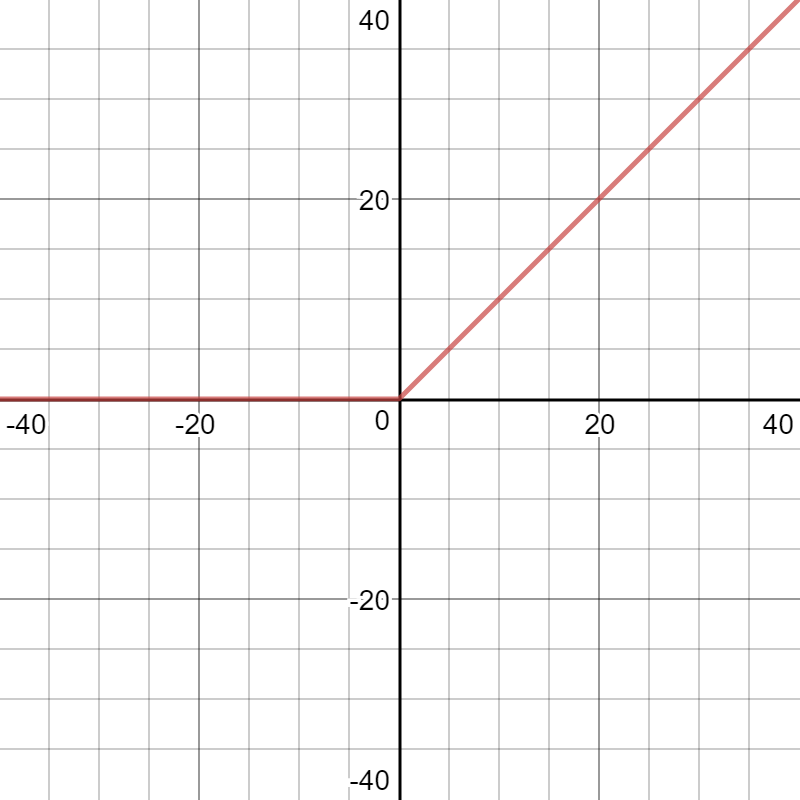
\includegraphics[width=.4\textwidth]{figures/relu}
	\caption{Graf aktivačnej funkcie ReLu.}
	\label{relu}
\end{figure}
ReLu je definovaná ako \[g(x) = max(0, x)\]
Pričom obor hodnôt je \(H = <0, \infty)\).

Trénovanie modelu je realizované v troch krokoch.
Výpočty sú vykonávané na dávkach dát.
V prvom kroku je vytvorená predikcia výsledku.
Následne sú tieto výsledky porovnané s očakávanými výstupmi a vypočíta sa chyba.
Táto chyba je vstupom do optimalizátoru, ktorý upraví premenné siete.
Celý proces sa opakuje vo viacerých epochách pre dosiahnutie väčšej presnosti.

Na výpočet rozdielu medzi výstupom neurónovej siete a predpokladaným výstupom využijeme krížovú entropiu.
Krížová entropia pre dve diskrétne rozdelenia pravdepodobností \(p\) a \(q\) je definovaná ako \[H(p,q) = - \sum p(x)\log q(x)\]

Optimalizovanie premenných modelu, čiže váhových matíc a prahov excitácie zabezpečí algoritmus spätného šírenia chyby.
Konkrétne ide o modifikáciu algoritmu Gradient Descent.

\section{Implementácia}
Model klasifikátora a jeho trénovanie je implementované v jazyku python, využitím modulu TensorFlow.
TensorFlow obsahuje mnoho algoritmov strojového učenia, preto nás oslobodzuje od ich implementovania.
Ďalšou výhodou tohto modulu je to, že separuje výpočty od pythonu, preto sú tieto výpočty rýchlejšie a je možné ich paralelizovať.
Program pozostáva z dvoch krokov, vytvorenie výpočtového grafu a jeho spustenie.
Výpočtový graf obsahuje celý model neurónovej siete spolu so všetkými výpočtovými krokmi pre trénovanie.

Vďaka tomu je možné implementovať funkciu pre trénovanie len niekoľkými riadkami.
\begin{minted}{python}
with tf.Session() as sess:
	sess.run(tf.global_variables_initializer())
	for epoch in range(hm_epochs):
		for _ in range(num_examples/batch_size):
			epoch_x, epoch_y = next_batch(batch_size)
			sess.run([optimizer, cost], 
				feed_dict={x: epoch_x, y: epoch_y})
\end{minted}

Na začiatku je nutné nainicializovať premenné, až potom je možné s nimi pracovať.
V každej epoche sú prejdené všetky dáta a sú optimalizované premenné siete.
Výpočty sa spúšťajú príkazom run.
Jeho parametrami sú výpočty, vrcholy TensorFlow grafu, a vstupné premenné potrebné pre tieto výpočty.
Optimizer je verzia algoritmu Gradient Descent.
\begin{minted}{python}
optimizer = tf.train.AdamOptimizer().minimize(cost)
\end{minted}
Na výpočet chyby (cost) je využitá TensorFlow implementácia krížovej entropie.
\begin{minted}{python}
prediction = neural_network_model(x)
cost = tf.reduce_mean(tf.nn.softmax_cross_entropy_with_logits(
			logits=prediction, 
			labels=y))
\end{minted}

%\chapter{Používateľské rozhranie}
\label{pouzivatelske_rozhranie}

Pre kontrolu funkčnosti nášho systému postačuje aj zmena zdrojových kódov.
Pre lepšiu použiteľnosť by však bolo vhodné vytvoriť nejaký druh prostredia pre používateľa.
Pre lepšiu prácu s naším systémom sme vytvorili grafické používateľské rozhranie.

Na začiatku nášho návrhu bola analýza už existujúcich programov, ktoré majú podobnú funkcionalitu.
Nakoľko systém, ktorý by generoval obrázky z hudobných skladieb neexistuje, ako predloha nám slúžila aplikácia Deep Dream Generátor, ktorá upravuje obrázky použitím algoritmov strojového učenia.

\section{Konceptuálny model}
Po analýze existujúcich riešení sme sa rozhodli, že naše grafické rozhranie bude poskytovať možnosť výberu skladby a následného výberu úseku skladby, z ktorého sa má generovať obrázok.
Na obrázku \ref{kon_model} je vidieť, že používateľ ("Človek") má prístup do galérie s obrázkami, ktoré môže mazať podľa svojho uváženia.
\begin{figure}[!ht]
	\centering 
	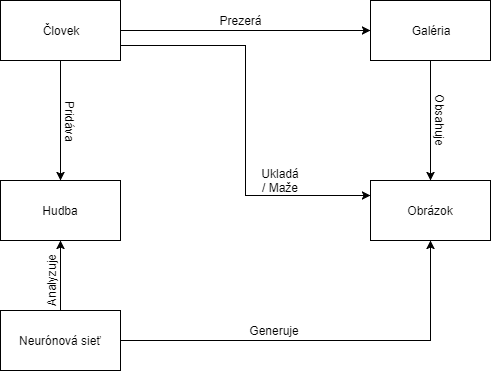
\includegraphics[height=.5\textwidth]{figures/km} 
	\caption{Konceptuálny model.} 
	\label{kon_model}
\end{figure}
Z tohto modelu je jasné, že generovanie obrázkov je priamočiare.
Človek vyberie hudbu, podľa ktorej sa má generovať, a náš systém, ktorý využíva neurónovú sieť, analyzuje skladbu a následne vygeneruje nový obrázok, ktorý sa uloží do galérie.

\section{Diagram postupnosti obrazoviek}

\begin{figure}[!ht] 
	\centering 
	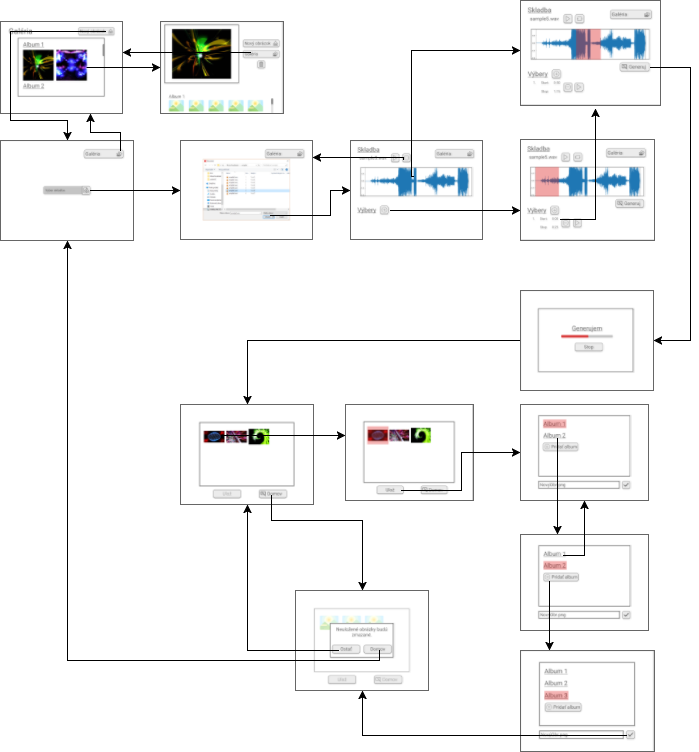
\includegraphics[height=.5\textwidth]{figures/ssq} 
	\caption{Diagram postupnosti obrazoviek.} 
	\label{ssq}
\end{figure}

Náš návrh je prehľadne vidno na diagrame postupnosti obrazoviek (Obr. \ref{ssq}).
Pri spustení sa otvorí stránka s galériou, z ktorej následne je možné prejsť na samotné generovanie nových obrázkov.
Proces vytvárania je rozdelený na tri sekcie, výber skladby, nastavenia úsekov skladby, podľa ktorých sa generovanie uskutočňuje, a samotné generovanie.
Po vytvorení nových obrázkov má používateľ možnosť uloženia do albumu.
V ponuke má zoznam už existujúcich albumov, no môže vytvoriť aj nový album.

\section{Iteratívny vývoj v prototypoch}
Návrh používateľského rozhrania sme vytvárali v dvoch cykloch.
Prototypy boli vytvorené pomocou nástroja Figma.
Každý prototyp bol otestovaný, a pre každý bolo vypočítané skóre použiteľnosti.

Oba prototypy testovali traja rôzny ľudia.
Vzorku účastníkov testu tvorili 20 až 25 roční študenti, ktorí nemali znalosti o tom ako má systém fungovať.
Priemerné skóre použiteľnosti pre prvý prototyp bolo 43,3 a pre druhý 55.

Po prvom testovaný nám bolo jasné, že používatelia nerozumeli nepopísaným tlačidlám a mali problém sa zorientovať na úvodnej ploche.
Po úpravách sa skóre rozhrania zlepšilo ale bolo stále jasné, že bežný používateľ nerozumie slovníku, ktorý sme použili a nevie čo má robiť.
Pri vytváraní finálneho funkčného prototypu sme sa snažili vyhnúť všetkým problémom a zlepšiť zrozumiteľnosť systému.


Vytvorenie prototypov a testovanie nám dalo lepšiu predstavu ako má finálny produkt vyzerať aby bol použiteľný.
Zároveň sme zistili, že chápanie systému, aj napriek jeho minimalistickému rozhraniu, je pre bežných používateľov prakticky neexistujúce.
Využitie metódy testovania použiteľnosti nám ale pomohlo rýchlo nájsť nedostatky v našom návrhu a zlepšiť celkovú kvalitu grafického používateľského rozhrania.

%% !TEX root = ../thesis.tex

\chapter{Syntetická časť práce}

% lorem ipsum
\blindtext
\blinditemize
\Blindtext
\Blindtext

%% !TEX root = ../thesis.tex

\chapter{Vyhodnotenie}

% lorem ipsum
\blindtext
\blinditemize
\Blindtext
\Blindtext

%% !TEX root = ../thesis.tex

\chapter{Záver}

% lorem ipsum
\Blindtext


% good linebraking of bibtex url
\setcounter{biburllcpenalty}{7000}
\setcounter{biburlucpenalty}{8000}

%% The bibliography
\phantomsection
\addcontentsline{toc}{chapter}{Literatúra}
\printbibliography[title={Literatúra}]

% List of acronyms
\printglossary[type=\acronymtype,title={\acrlistname}]

%% Appendix
%% !TEX root = ../thesis.tex

\chapter*{Zoznam príloh}
\addcontentsline{toc}{chapter}{Zoznam príloh}

\begin{description}
	\item[Príloha A] Lorem ipsum
    \item[Príloha B] CD médium -- záverečná práca v~elektronickej podobe,
    \item[Príloha C] Používateľská príručka
    \item[Príloha D] Systémová príručka
\end{description}

%\appendix
%\renewcommand\chaptername{Príloha}
%% !TEX root = ../thesis.tex

\chapter{Lorem ipsum}

\blindtext
\newpage
\blindtext


% zivotopis autora
%\curriculumvitae\protect
%Táto časť\/ je nepovinná. Autor tu môže uviesť\/ svoje biografické
%údaje, údaje o~záujmoch, účasti na~projektoch, účasti na~súťažiach,
%získané ocenenia, zahraničné pobyty na~praxi, domácu prax, publikácie
%a~pod.

\end{document}
